\documentclass{article}
\usepackage{realtristan}
\title{Chemistry}
\author{Tristan Simpson}
\begin{document}
\maketitle
\tableofcontents

\section{Atoms and Molecules}
\begin{itemize}
    \item An atom is the smallest unit of an element.
    \item A molecule is a group of atoms bonded together.
\end{itemize}

\section{Inter and Intramolecular Forces}
\begin{itemize}
    \item The \textbf{intramolecular} force is what holds the atoms together.
    \item The \textbf{intermolecular} force is what holds the molecules (a group of atoms bonded together) together.
\end{itemize}
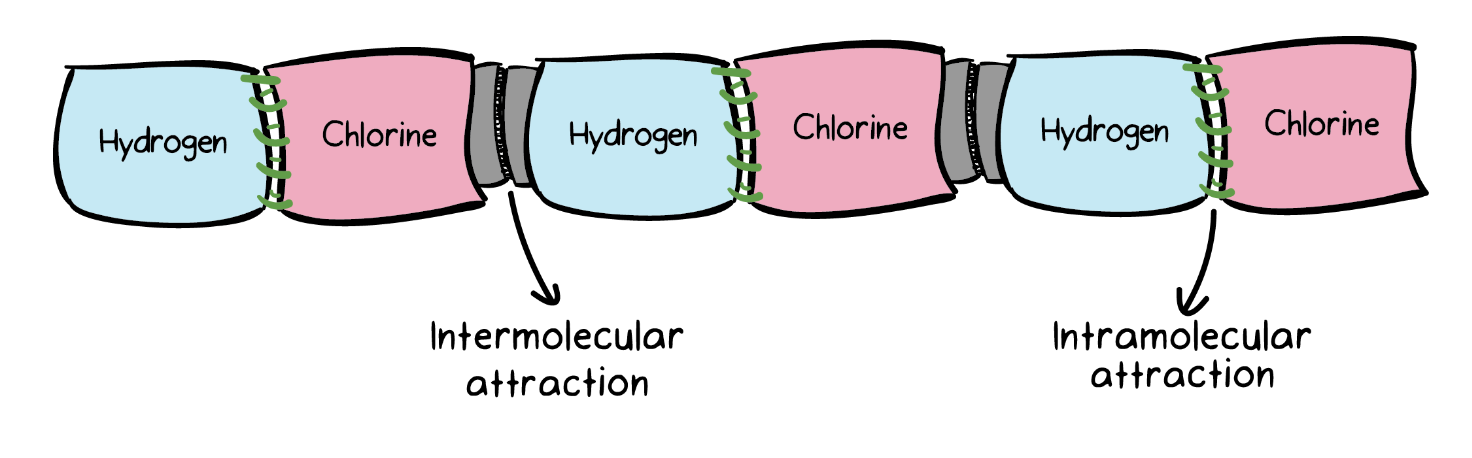
\includegraphics[scale=0.33]{images/molecularforces.png}


\end{document}